As described earlier, subtopic clustering has always been a challenging task in information retrieval field. The subtopic retrieval method developed by Bernardini et al. is limited by several factors: 
\begin{itemize}
    \item It is highly dependent on keyphrases generated from the search results
    \item In high precision scenario where our candidate set size is small, it will be difficult to generate useful keyphrases
    \item Their method is evaluated with a non-standard evaluation metric
\end{itemize}
Hence we feel, the problem of subtopic clustering requires a generic solution which can be verified by standard clustering metrics. Transformer based embedding model brings not only simplicity, efficiency and generality of an embedding model but also the ability to capture complex semantic information. Both of these features are necessary key-ingredients to solve challenging IR problems such as subtopic clustering. Our main focus in this section is to use these embeddings as key ingredients and find simple modifications that can capture subtopic similarity between passages related to a topic and thus can cluster them based on those subtopics.

\subsection{Basic steps to subtopic clustering} We model subtopic clustering task as a pairwise distance learning problem. Any subtopic clustering problem can be solved by two basic steps:
\begin{itemize}
    \item Step 1: Estimate pairwise distance between all passage pairs.
    \item Step 2: Use Hierarchical Agglomerative clustering with the pre-computed pairwise distance to generate clusters of passages.
\end{itemize}

We focus on Step 1 to develop a suitable pairwise similarity metric between passages.

\subsection{Transformer embeddings} In their Sentence-BERT work, authors generate fixed length embeddings for a given word sequence. Dor et al. \cite{dor2018learning} propose triplet fine-tuning technique which trains the embeddings to be better suited in predicting similarity of sentence pairs based on their likeliness of sharing same section in an Wikipedia article. Each training sample consists of one anchor sentence, one similar sentence which is from same section than the anchor and one dissimilar sentence which is from different section than anchor. Using each of these approaches, we obtain fixed length embeddings for passages using tokenized passages as input token sequence. A straight-forward way to solve the subtopic clustering problem is to use cosine similarity between these fixed length vectors as pairwise similarity between passages and feed to a clustering algorithm to obtain subtopic clusters. Note that, transformer models have a maximum input length. So for longer passages, we may truncate extra tokens beyond the maximum length. 

Although the triples data and target task proposed by Dor et al. may help detecting a sentence pair from same section of Wikipedia, we hypothesize that without certain modifications specific to subtopic clustering, we obtain sub-optimal results. There are several reasons behind our hypothesis: 
\begin{itemize}
    \item Natural sentences are shorter compared to passages and henceforth, it is hard to find sentences with much topical drifts. So there is hardly any ambiguity in deciding the central topic discussed in an article. So the target task for sentence-pair similarity is to decide whether the two specific topic discussed in a pair of sentences should be discussed in same section or they are distinct enough to be on different sections of an article. For passage-pair however it is much more difficult because constituent sentences in a passage may be of different fine-grained topic.
    \item Wikipedia articles are organized in hierarchical sections; passages in deeper hierarchy tend to discuss more specific topics than passages in higher level. Hence two passages which share the same top-level section but belongs to different deeper level section may provide ambiguous supervision signals if used as training samples to fine-tune a model. This hierarchical ambiguity in training data generation is not considered in Dor et al. method which may result to undertrained model if adapted for subtopic clustering of passages.
    \item As any subtopic clustering is highly query dependent, we hypothesize that an accurate subtopic similarity metric must take the current query into consideration as context information.
\end{itemize}

We propose the following simple modifications to the previous approaches when applied to subtopic clustering:
\begin{itemize}
    \item Due to the reason discussed above, while generating passage triples for fine-tuning, we consider only passages which are from different highest level hierarchy than the anchor passage in to be considered dissimilar. This will provide clear, unambiguous and distinguishable supervision signal to the model under fine-tuning and help it to quickly learn the desired similarity function. Figure \ref{fig:conv} depicts the training data generation.
    \item We train a query-dependent shallow network to provide pairwise passage similarity scores which are used by subsequent clustering algorithm to generate subtopic clusters of passages. Next we discuss this approach in more detail.
\end{itemize}{}
\begin{figure}[h]
  \centering
  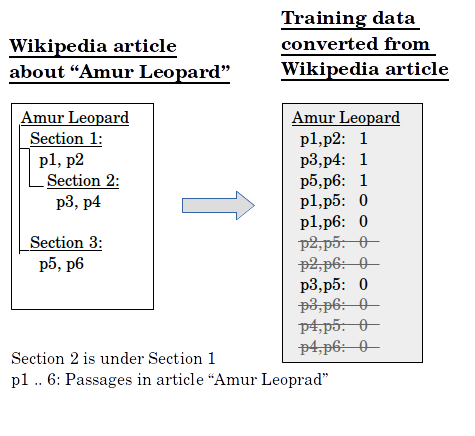
\includegraphics[width=\linewidth]{graphics/car_y1_conv.png}
  \caption{Training data generation from Article \textit{Amur Leopard} and balancing the dataset (depicted in grey strikethrough)}
  \label{fig:conv}
\end{figure}

\subsection{CATS: Context Aware Triamese Similarity network}\label{sec:cats} Similarity between a pair of texts is often subject to a context. In context of \textit{endangered species}, a pair of passages about \textit{Amur leopard} and \textit{Vaquita porpoise} should be considered similar. However this is not the case if the context changes to \textit{bycatch}. In subtopic clustering problems, context plays an important role in deciding whether passages about same broad topic should share the same subtopic cluster or not. Keeping this in mind, we propose CATS, Context Aware Triamese Similarity network, a triamese shallow network which learns a similarity function between a pair of passage embeddings given a third embedding vector containing context information. For our implementation, we use the topic title as our context information.

As depicted in Figure \ref{fig:triam}, the general CATS architecture consists of three identical fully connected triamese neural layers ($DL1$), meaning they share the same weights. Each of them accepts fixed length embedding vectors of context and pair of passages respectively ($u,v,w$). Due to their triamese nature, they project all three embedding vectors to the same embedding subspace. The projected vectors ($u',v',w'$) and their difference vectors ($(v'-w'),(v'-u'),(w'-u')$) are concatenated. The concatenated output vector is sent through another fully connected neural layer ($DL2$) which emits a similarity score.
\begin{figure}[h]
  \centering
  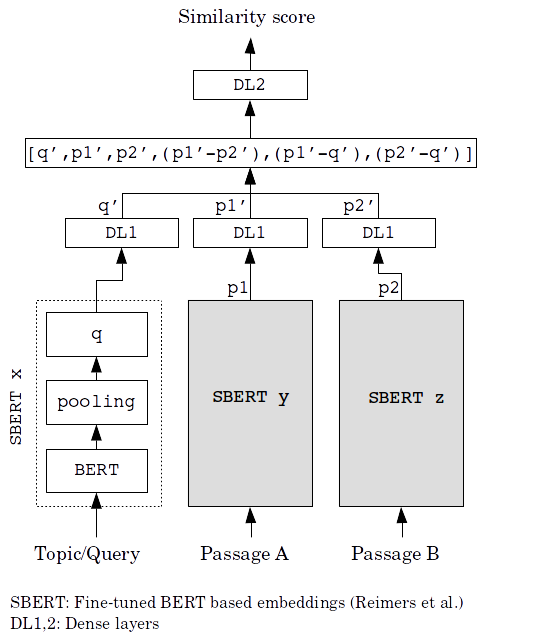
\includegraphics[width=\linewidth]{graphics/triamese.png}
  \caption{Triamese network used to estimate query dependent pairwise passage similarity score used for subtopic clustering}
  \label{fig:triam}
\end{figure}

\subsection{Finetuning transformers for sequence pair tasks} Fine-tuning is a crucial step in training Transformer models because this allows the model to be specifically suited for a particular downstream task. In the original BERT work, the BERT model is fine-tuned for a binary classification task with STSB benchmark dataset. In that work BERT model is fine-tuned for next sentence prediction task where given a sentence-pair, the model has to predict whether the second sentence should follow the first sentence. We fine-tune transformer with a modified task: given a passage-pair, predict whether they should belong to the same subtopic. This modified task setting allows us to use output of the model as the similarity score between the input passages. However, our focus for this work is to explore utilization of fixed sized passage embeddings and hence use this technique only as a strong baseline against our embedding based methods.